\documentclass[11pt,titlepage]{article}
\usepackage[reqno]{amsmath}
\usepackage{amssymb}
\usepackage{epsf}
\usepackage{epsfig}
\usepackage{url}

% === additional commands/packages/settings ===
\usepackage{graphicx,psfrag,natbib}
\usepackage{setspace}
\usepackage{vmargin}
\setpapersize{USletter}

% === dcolumn package ===
\usepackage{dcolumn}
\newcolumntype{.}{D{.}{.}{-1}}
\newcolumntype{d}[1]{D{.}{.}{#1}}

% === newcommands from sei.tex ===
\newcommand{\EI}{\ensuremath{{\mathfrak EI}}}
\newcommand{\Tiny}{\tiny}
\newcommand{\sump}{\sum_{i=1}^p}
\newcommand{\mean}{\frac{1}{p}\sump}
\newcommand{\ub}{\Dot{\beta}}
\newcommand{\ut}{\Dot{\theta}}
\newcommand{\bbeta}{{\mathfrak B}}
\newcommand{\btheta}{{\mathfrak T}}
\newcommand{\blambda}{{\mathfrak L}}
\newcommand{\bbetau}{\breve{\mathfrak B}}
\newcommand{\bV}{{\cal V}}
\newcommand{\sigmau}{\breve{\sigma}}
\newcommand{\Sigmau}{\breve{\Sigma}}
\newcommand{\rhou}{\breve{\rho}}
\newcommand{\psiu}{\breve{\psi}}
\newcommand{\Eu}{\breve{\text{E}}}
\newcommand{\Vu}{\breve{\text{V}}}
\newcommand{\Bb}{B^b}
\newcommand{\Bw}{B^w}
\newcommand{\NbD}{{N_i^{bD}}}
\newcommand{\NwD}{{N_i^{wD}}}
\newcommand{\NbR}{{N_i^{bR}}}
\newcommand{\NwR}{{N_i^{wR}}}
\newcommand{\NbN}{{N_i^{bN}}}
\newcommand{\NwN}{{N_i^{wN}}}
\newcommand{\tp}{{\mbox{\Tiny{+}}}}
\newcommand{\NpD}{{N_i^D}}
\newcommand{\NpR}{{N_i^{R}}}
\newcommand{\NpN}{{N_i^{N}}}
\newcommand{\Nbp}{{N_i^{b}}}
\newcommand{\Nwp}{{N_i^{w}}}
\newcommand{\Npp}{{N_i}}
\newcommand{\Nppp}{{N}}
\newcommand{\Nbpp}{{N^{b}}}
\newcommand{\Nwpp}{{N^{w}}}
\newcommand{\sumpN}{\sump\Npp}
\newcommand{\NsumpN}{\frac{1}{\Nppp}\sumpN}
\newcommand{\nbp}{{N_i^{bT}}}
\newcommand{\nwp}{{N_i^{wT}}}
\newcommand{\npp}{{N_i^{T}}}
\newcommand{\NbV}{{N_i^{bT}}}
\newcommand{\NwV}{{N_i^{wT}}}
\newcommand{\NpV}{{N_i^{T}}}
\newcommand{\xb}{\bar{X}}
\newcommand{\wb}{\bar{W}}
\newcommand{\tb}{\bar{T}}
\newcommand{\cx}{{\mathbb X}}
\newcommand{\cw}{{\mathbb W}}
\newcommand{\ct}{{\mathbb T}}
\newcommand{\cpij}{{\mathbb P}^*_{ij}}
\newcommand{\cpi}{{\mathbb P}^*_i}
\newcommand{\cwd}{{\dot{\mathbb W}}}
\newcommand{\ctd}{{\dot{\mathbb T}}}
\newcommand{\cxd}{{\dot{\mathbb X}}}
\newcommand{\cxb}{\bar{\mathbb X}}
\newcommand{\cz}{{\mathbb G}}
\newcommand{\ch}{{\mathbb H}}
\newcommand{\cm}{{\mathbb M}}
\newcommand{\E}{{\textbf{E}}}
\newcommand{\V}{{\textbf{V}}}
\newcommand{\C}{{\textbf{C}}}
\newcommand{\rE}{{\text{E}}}
\newcommand{\rV}{{\text{V}}}
\newcommand{\rC}{{\text{C}}}
\newcommand{\TN}{\text{TN}}
\newcommand{\BN}{\text{BN}}
\newcommand{\N}{\text{N}}
\renewcommand{\P}{\text{P}}
\newcommand{\D}{\textbf{D}}
\newcommand{\R}{\ensuremath{\textbf{R}}}
\newcommand{\Rr}{\ensuremath{\{\textbf{R}\diagdown r}\}}
\newcommand{\bC}{\ensuremath{\textbf{C}}}
\newcommand{\Cc}{\ensuremath{\{\textbf{C}\diagdown c}\}}
\newcommand{\one}{{\mathbf{1}}}
\newcommand{\Q}{\ensuremath{\overset{\vspace{3em}}{\text{\Huge ?}}}}
\newlength{\padsp}
\settowidth{\padsp}{$(\beta^w_i=\nwp/\Nwp)$}
\newcommand{\padbw}{\hspace*\padsp}
\newcommand{\bkappa}{\boldsymbol{\kappa}}

\newcommand{\bb}{\beta^{\text{bad}}}
\newcommand{\bg}{\beta^{\text{good}}}
\renewcommand{\bibitem}{\vskip 2pt\par\hangindent\parindent\hskip-\parindent}

\title{Analyzing Second-Stage Ecological Regressions: Extensions to
  Herron and Shotts}

\author{Christopher Adolph\thanks{Ph.D. candidate, Department of
    Government, Harvard University. (Littauer Center---North Yard,
    Harvard University, Cambridge MA 02138;
    \texttt{http://chris.adolph.name},
    \texttt{cadolph@Fas.Harvard.Edu}).}
\and %
Gary King\thanks{Professor of Government, Harvard University and
  Senior Science Advisor, World Health Organization (Center for Basic
  Research in the Social Sciences, 34 Kirkland Street, Harvard
  University, Cambridge MA 02138; \texttt{http://GKing.Harvard.Edu},
  \texttt{King@Harvard.Edu}, (617) 495-2027).}  }

\begin{document}
\maketitle
% \begin{abstract}
%   Herron and Shotts make an important contribution by 
%   noting that the interesting point that 
%   the only time the fully adjusted procedure clearly dominates least
%   squares regression is when the bounds are uninformative and
%   ecological inference is so risky that, unless additional information
%   was available, no analysis should be trusted at all.
% \end{abstract}

\section{Introduction}

We take this opportunity to comment on Herron and Schotts' article
(hereinafter HS) because of its potential to affect the way a
considerable body of practical research is conducted, and because of
HS's interesting and productive ideas.  HS's paper is based on the
suggestions in three paragraphs in King (1997: 289--90).  Since these
paragraphs were not summarized in HS, we thought they might be a
useful place to start:
\begin{quotation}
  If a second stage analysis is conducted, least squares regression
  should probably not be used in most cases, even though it may not be
  particularly misleading.  The best first approach is usually to
  display a scatterplot of the explanatory variable (or variables)
  horizontally and (say) an estimate of $\beta_i^b$ or $\beta_i^w$
  vertically.  In many cases, this plot will be sufficient evidence to
  complete the second stage analysis.
  
  If it proves useful to have more of a formal statistical approach,
  and many of the actual values of $\beta_i^b$ fall near zero or one,
  then some method should be used that takes this into account.  The
  data could be transformed, via a logit or probit transformation, or
  [the ``extended model''] could be applied\ldots.  Whatever method is
  chosen, the researcher should be careful to include the fact that
  some estimates of $\beta_i^b$ are more uncertain than others.
    
  In practice, a weighted least squares linear regression may be
  sufficient in many applications, with weights based on the standard
  error of $\beta_i^b$ (or other quantity of interest).  Researchers
  should be careful in applying this simplified method here, and
  should verify its assumptions with scatterplots. \ldots This is not
  as theoretically elegant a procedure as the more formal set up in
  [the ``extended model''] but it is simple, relatively robust, and
  probably complete enough to be of use in many applications.
\end{quotation}  

HS add to the ideas in these paragraphs by pointing out that
precinct-level estimates from EI regress to the mean.  This
``shrinkage'' property is indeed a characteristic of EI, as it is for
all Bayesian models (of which EI is one).  This shrinkage results in
optimal estimates, in terms of generating estimates with the smallest
possible mean square error.  Thus, we agree with the implication of
HS's article that the best possible estimate of $\beta^b_i$, under
HS's assumptions, is that produced by EI.  But HS also make the
interesting and correct point that using Bayesian mean posterior
estimates with this property, like those given by EI, as dependent
variables in least squares regression can, under some circumstances,
produce biased estimates.  This central point of HS's paper is an
important contribution and one on which we build here.

Instead of least squares regression, HS's suggested procedure is to
use a bias adjusted slope for the second stage regression but to leave
the constant term unchanged.  Their adjustment is based on linear
approximations within the classical linear econometric theory
framework.  The problems we describe below with HS's approach are all
due assuming linearity when modeling an inherently nonlinear and
bounded relationship, as well as not completing the task they set for
themselves within this framework.

We replicated HS's simulations without trouble.  We then examined how
well their adjusted regression procedure fit the observed data based
on $\hat\beta_i^b$ and the true (normally unobserved) $\beta_i^b$.  We
find that correcting the slope but not the constant, as HS suggest, is
considerably worse than an unadjusted regression of $\hat\beta_i^b$ on
$Z$ and every other procedure discussed in HS's paper and the
literature we have examined.  The regression line from HS's method
usually misses the cloud of true $\beta_i^b$ points by a wide margin.

We therefore begin by extending HS's partial adjustment procedure,
within their linear regression framework, by developing an adjustment
for the constant term also.  Our fully adjusted second stage
regression method naturally extends HS's framework and dominates HS's
procedure.  We also compare our fully adjusted procedure to unadjusted
linear regression and find four prototypical situations likely to
arise in practice.  Since each situation is easily detectable from the
available aggregate data, users will know which situation they are in
and can take the appropriate action.  As it turns out, the HS
partially adjusted procedure is never called for.  The fully adjusted
procedure is best only for data with bounds so wide that making any
ecological inferences at all in the first stage is inadvisable (unless
one has strong auxiliary information), due to extreme model
dependence.  In the other three situations, the best procedures are
unadjusted least squares, unadjusted weighted least squares
regression, and a logistic regression procedure, respectively.

\section{A Fully Adjusted Second Stage Regression Procedure}
\label{s:fulladj}

HS consider models in which a researcher wishes to regress an EI-based
estimate, $\hat\beta_i^b$, on some explanatory variable $Z_i$:
\begin{equation}
  \label{eq:ssreg}
  \hat\beta_i^b=\alpha_U+\gamma_U Z_i + \nu_i,
\end{equation}
They argue that unless the measurement error in $\hat\beta_i^b$ is
uncorrelated with the true $\beta_i^b$, $\gamma_U$ will be biased.
Strictly speaking, this (typically downward) bias will be limited in
the presence of tight bounds on the estimates of $\hat\beta_i^b$.
However, to the extent that the bounds are wide and the linearity
assumed by Eq. \ref{eq:ssreg} holds, $\hat\gamma_U$ will be an
underestimate of the true $\gamma$, which HS denote $\gamma_R$.

HS propose a correction for this attenuation bias based on the
assumption that the measurement error in $\hat\beta_i^b$ is a linear
function of the true $\beta_i^b$'s:
\begin{equation}
  \label{eq:hserr}
  \hat\beta_i^b - \beta_i^b = \delta_0^b + \delta_1^b\beta_i^b + \zeta_i.
\end{equation}
If this assumption holds, then it is easy to show that the true slope,
$\gamma_R$, can be calculated as $\gamma_U/(1 + \delta_1^b)$; HS label
this adjustment $\gamma_A$.  However, the same method shows that the
intercept $\alpha$ should be adjusted, so that $\alpha_A =
(\alpha_U-\delta_0^b)/(1+\delta_1^b)$.  Besides being consistent with
HS's slope adjustment, intercept correction also makes intuitive
sense.  Unless the mean of $Z$ is approximately zero, inflating the
slope without changing the intercept can produce much higher or lower
predictions of $\hat\beta_i^b$ from Eq.  \ref{eq:ssreg} than are
consistent with the data, or even possible.  Only when $\bar Z \approx
0$ is the unadjusted $\alpha$ approximately right.

Since we can easily adapt the procedure HS recommend in Section 7.2
to produce estimates of both $\delta_0^b$ and $\delta_1^b$, researchers
can make a full adjustment of a second-stage regression as easily as a
partial adjustment.
\begin{table}[tb]
\label{t:hsrep}
\begin{center}
\begin{tabular}{cc|c c c}
Model Parameters & Truth & \multicolumn{3}{c}{Estimates} \\
$\breve\psi$  & $\gamma_R$ & $\hat\gamma_R$  &       $\hat\gamma_U$ & $\hat\gamma_A$ \\\hline
(0.5, 0.5, 0.1, 0.1, 0)&1 &       0.04    &       0.02    &       0.04        \\
(0.75, 0.5, 0.1, 0.1, 0) &1       &       0.04    &       0.02    &       0.04        \\
(0.75, 0.75, 0.1, 0.1, 0) &1      &       0.04    &       0.02    &       0.04     \\
(0.9, 0.9, 0.1, 0.1, 0) &1&       0.02    &       0.01    &       0.02          \\
(0.5, 0.5, 0.32, 0.1, 0) &1       &       0.19    &       0.13    &       0.19        \\
(0.6, 0.6, 0.1, 0.32, 0) &1       &       0.04    &       0.01    &       0.04     \\
(0.9, 0.1, 0.32, 0.32, 0)&1       &       0.15    &       0.08    &       0.15        \\
(0.5, 0.5, 0.1, 0.1, 0.3)&1       &       0.04    &       0.02    &       0.04     \\
\hline
\end{tabular}
\end{center}
\caption{\em Estimated and ``true'' slopes from 
second-stage regressions based on Herron and Schott's Monte Carlo 
procedure. This table replicates the results of simulations presented in
HS Table 2.  All results are averages over 100 simulations.  
The difference and ratios presented in HS Table 2 were also 
successfully replicated, and are not shown here.}
\end{table}

\section{Herron and Shotts' Monte Carlo Simulations}

The Monte Carlo procedure used to generate results by HS is
inappropriate to the task of evaluating second stage regressions.  HS
draw $\beta_i^b$ from the EI model without covariates.  Then they
create the covariate for the second stage $Z_i$ endogenously as equal
to $\beta_i^b$ plus random noise.  The problem with this procedure is
that it induces immense attenuation bias due to random measurement
error in the explanatory variable, quite apart from any attenuation
bias that may occur due to the Bayesian shrinkage error in the EI
estimate.

This can be seen by studying the parameters of the model they created
from which to draw their Monte Carlo data.  In this model, the slope
of the coefficient on the covariate in the second regression is 1 (in
their notation, $\gamma_R=1$).\footnote{Under the HS Monte Carlo
  setup, $E(\beta_i^b)=E(\alpha+\gamma_R Z_i)$, where
  $Z_i=\beta_i^b+\tau_i$ and $E(\tau_i)=0$.  Hence
  $E(\beta_i^b)=\alpha+\gamma_RE(\beta_i^b+\tau_i)=\alpha+\gamma_R\beta_i^b$.
  which implies that $\alpha=0$ and $\gamma_r=1$.}  However, the
estimates of this slope from their simulations of the true $\beta_i^b$
(i.e., without any attenuation bias in the dependent variable at all)
regressed on $Z$ gives a drastically biased estimate.  This slope
estimate does not appear in their article, but we were able to to
replicate their Table 2 exactly, and in our Table \ref{t:hsrep}
present these numbers.  As can be seen, whereas the theoretical value
of $\gamma_R$ is 1, estimates indicate that $\hat\gamma_R\approx
0.07$.  Thus, since the unadjusted method is unable to recover the
coefficients without shrinkage when using the true value of the
dependent variable, this Monte Carlo setup is certainly inappropriate
for assessing a dependent variable that is estimated.

A second problem with the Monte Carlo procedure employed by HS is that
it artificially rules out nonlinear relationships between $\beta_i^b$
and $Z_i$.  Perhaps the most common situation confronting users of
second-stage EI regressions is an unbounded independent variable which
covaries with a necessarily-bounded dependent variable, which is
estimated by EI.  By contrast, HS construct their explanatory
variable, $Z_i$, from the bounded $beta_i^b$'s (plus a normal
disturbance), effectively ensuring that the relationship between the
two is linear and contained within the (0,1) bound on $beta_i^b$.
Within this framework, it is simply not possible to test the
robustness of the HS adjustment to the sort of nonlinear relationships
which may crop up in applied research.

\section{An Improved Monte Carlo Simulation} \label{s:alt}

Our conclusions below do not depend on changing the simulation method,
but we do so in order to make the results more coherent.

To simulate, we follow the logic of the extended EI model.  Thus, we
first fix $X$, the covariates $Z$ (to values so that it is
uncorrelated with $X$), the values for the intercept and the slope
parameter on $Z_i$, and the variance and covariance parameters of the
truncated bivariate normal.  Then, for each simulation, we draw the
$\beta_i^b$'s from the extended EI model conditional on $X_i$ and
$Z_i$.  The assumption that $X_i$ and $Z_i$ are uncorrelated enables
us to run a (first-stage) basic EI model (i.e., with no covariates)
without inducing aggregation bias.  Unless the relationship is clearly
nonlinear because the bounds are very influential, a regression of the
true $\beta_i^b$ on $Z_i$ recovers the intercept and slope
coefficients accurately.

To facilitate replication, we present our simulation procedure in a manner comparable to HS:

\begin{enumerate}

\item Choose $\phi_1$, $\phi_2$, $\phi_3$, $\phi_4$, $\sigmau_b$,
$\sigmau_w$, and $\rhou$.

\item Repeat the following 100 times:

\begin{enumerate}
  
\item Draw $X_i$, $i=1,\ldots,500$ from the uniform distribution.
  Various ranges of uniform random numbers are chosen to produce
  different mixtures of wide and narrow bounds.
  
\item Draw $Z_i$ from the normal distribution.  Various means and
  variances are used in different scenarios.
  
\item Calculate the untruncated means $\bbetau^b_i$ and $\bbetau^w_i$
  from the extended EI model, as follows:
\begin{align}
  \bbetau^b_i &= \left[\phi_1(\sigmau_b^2+0.25)+0.5\right]
  +\phi_2Z_i^b\notag\\
  \bbetau^w_i &= \left[\phi_3(\sigmau_w^2+0.25)+0.5\right]
  +\phi_4Z_i^w
  \label{reparZ}
\end{align}

\item Draw $\beta_i^b$ and $\beta_i^w$ from the truncated bivariate
  normal given $\psiu =
  \(\bbetau^b,\bbetau^w,\sigmau_b,\sigmau_w,\rhou\)$.
  
\item Obtain estimates of $\hat\beta_i^b$ and $\hat\beta_i^w$ from EI,
  omitting the covariate $Z_i$.
  
\item Estimate $\hat\delta_0^b$ and $\hat\delta_1^b$ using Eq.
  \ref{eq:hserr}.
  
\item Estimate the following equations:
\begin{align}
  \beta_i^b=\alpha_R+\gamma_R Z_i + \nu_i \textrm{by LS}\notag\\
  \hat\beta_i^b=\alpha_U+\gamma_U Z_i + \nu_i \textrm{by LS}\notag\\
  \hat\beta_i^b=\alpha_W+\gamma_W Z_i + \nu_i \textrm{by WLS}
\end{align}

\item Finally, obtain adjusted slopes and coefficients according to
  the procedure described in Section \ref{s:fulladj}.

\end{enumerate}
\end{enumerate}


We use this Monte Carlo setup to illustrate four prototypical
situations that would seem to map out the space of applications in
which the various methods work in different ways.

First, when ecological data have very wide bounds, EI (and any method
of ecological inference) will be sensitive to modeling assumptions.
In many applications with data like these, no ecological inference
should be conducted unless one has some special auxiliary information
about the model assumptions.  If one proceeds to the second stage
anyway, then a researcher would find that the full adjustment is an
improvement: Indeed, only in this situation does the full adjustment
procedure correct appropriately for attenuation bias and dominate the
unadjusted procedure.  (This is the situation in which EI is closest
to linear regression, which makes HS's linear econometrics framework
most appropriate.)  Figure \ref{f:wide} plots the covariate $Z_i$
horizontally by the true $\beta_i^b$ (in the left graph) and the
estimated $\hat\beta_i^b$ (in the right graph) vertically.  Note how
the unadjusted least squares line (marked LS) fits the estimated
points well (in the right graph) but are attenuated for the true
points (in the left).  Since the bounds are all very wide, the
variances are almost constant and so the weighted least squares
(marked WLS) line is practically on top of the LS line.  In contrast,
the line representing the fully adjusted method we developed (marked
FA) fits the true points well, and hence corrects for the attenuation.
Figure \ref{f:wide} also plots Herron and Shotts' partially adjusted
method (marked HS), which is more biased than any of the
alternatives, a problem which grows in severity as the mean of $Z$
departs from zero.  Since Herron and Shotts' proposal is never better
than full adjustment, and often dramatically worse, we do not consider
it further.
\begin{figure}[t]
  \begin{center}
    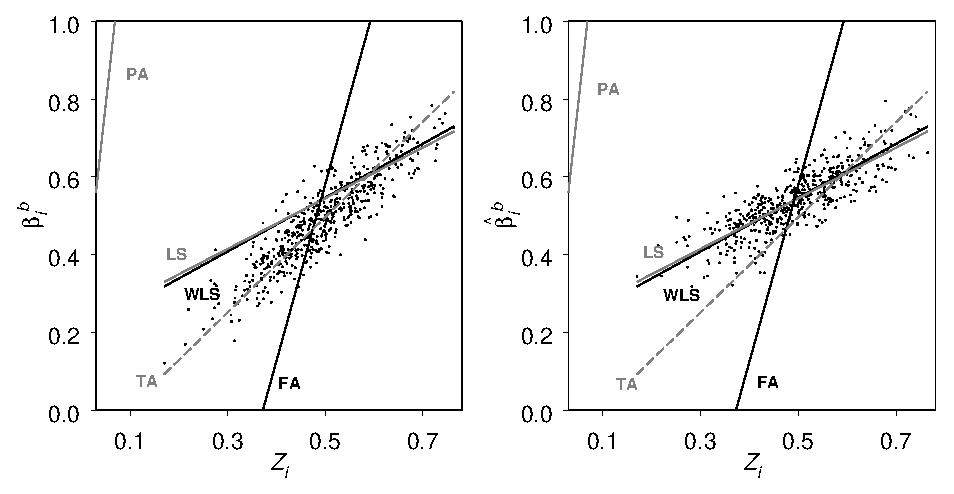
\epsfig{file=wide.eps}
    \caption{Data with Wide Bounds. Plot of $Z_i$ horizontally by
      the estimated $\hat\beta_i^b$ vertically (in the right graph)
      and the true $\beta_i^b$ (in the left graph), with fits for
      Herron and Shotts' partially adjusted procedure (HS), least
      squares (LS) and weighted least squares (WLS) almost on top of
      one another, and our fully adjusted method (FA).  Note how FA
      fits the true points best.  Data were generated from the
      extended EI model, with $\breve\psi=(-2,1,-2,1,0.05,0.05,0)$, $X
      \sim \textrm{Uniform}(0,0.2)$, and $Z \sim
      \textrm{Normal}(0.5,0.1)$.}
    \label{f:wide}
  \end{center}
\end{figure}

Second, when the bounds are at least somewhat informative (that is,
few of the bounds are extremely wide), we are in the situation when we
would be more likely to trust ecological inferences using EI (or
another method that takes into account the information in the
precinct-level bounds).  When the relationship is approximately (or
locally) linear, we find that ordinary least squares regression
usually does as well as, and often better than, the fully adjusted
procedure.  Figure \ref{f:narrow} gives one example where least
squares, weighted least squares, and our fully adjusted method all
give approximately the same estimates.
\begin{figure}[t]
  \begin{center}
    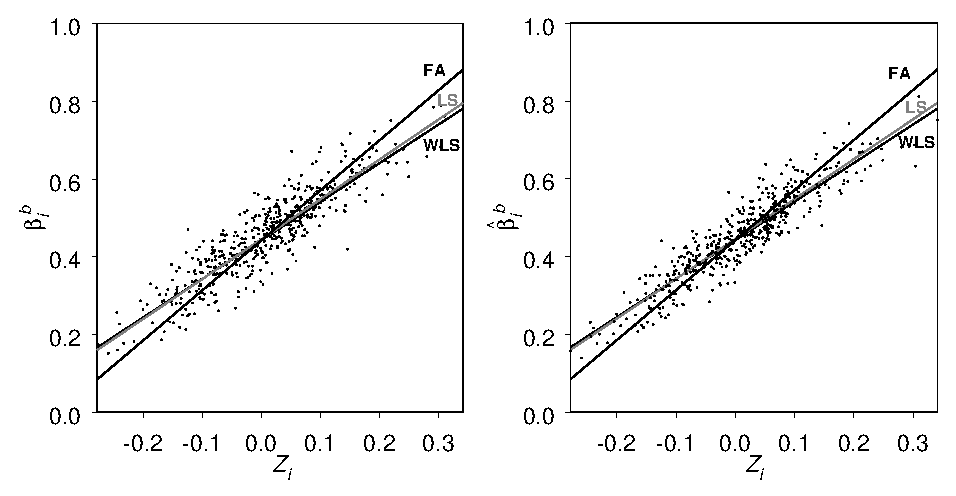
\epsfig{file=narrow.eps}
    \caption{Data with Informative Bounds. Plot of the $Z_i$ horizontally by
      the estimated $\hat\beta_i^b$ vertically (in the right graph)
      and the true $\beta_i^b$ (in the left graph) with fits for least
      squares (LS) and weighted least squares (WLS) appear almost on
      top of one another, and our fully adjusted method (FA).  Note
      how all three methods give almost the same answer. Data were
      generated from the extended EI model, with
      $\breve\psi=(-0.2,1,0.6,1,0.05,0.05,0)$, $X \sim
      \textrm{Uniform}(0.2,1)$, and $Z \sim \textrm{Normal}(0,0.1)$.}
    \label{f:narrow}
  \end{center}
\end{figure}

Third, when some observations have wide bounds and others have narrow
bounds, and $\hat\beta_i^b$ is an approximate (or locally) linear
function of $Z_i$, (unadjusted) weighted least squares (WLS)
regression will often be substantially less biased than unadjusted
regression, and be approximately equivalent to and often better than
the fully adjusted procedure (although like all weighted regressions,
this procedure would have higher variance than the unadjusted
procedure).\footnote{HS studied consistency, and implicitly bias, but
  did not address other properties, such as efficiency.  A full
  evaluation should of course consider these properties as well.}
This is contrary to HS's claims that WLS would not make a difference;
what they missed by applying a linear regression framework to this
problem with bounds and nonlinearity is that the degree of attenuation
is directly related to the width of the bounds --- as can be seen by
the differences between Figures \ref{f:wide} and \ref{f:narrow} ---
and so the weights are correlated with the attenuation bias and can
effectively adjust for it.  Figure \ref{f:mixed} provides an example
of this phenomenon.  We generated the data for this figure from the
same model as the other figures, changing only the parameter values so
that the points were affected by the bounds.  The effect of the wide
bounds on some observations can be seen by the attenuation in the set
of points forming a flatter slope in the right graph (as compared to
the left graph which has no such feature).  As a result the least
squares (LS) line is a good deal flatter than it should be (as judged
by the fit to the points in the left graph).  In this example, the
fully adjusted (FA) and the weighted least squares (WLS) lines both
correct for most of the attenuation.
\begin{figure}[t]
  \begin{center}
    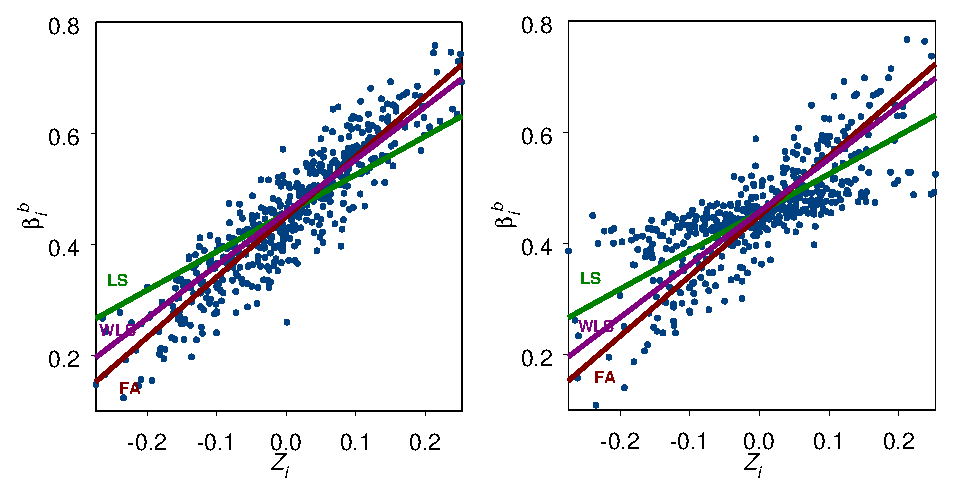
\epsfig{file=mixed.eps}
    \caption{Data with Narrow and Wide Bounds. Plot of the $Z_i$ 
      horizontally by the estimated $\hat\beta_i^b$ vertically (in the
      right graph) and the true $\beta_i^b$ (in the left graph) with
      fits least squares (LS), weighted least squares (WLS), and our
      fully adjusted method (FA).  Note how (unadjusted) WLS corrects
      for most of the attenuation bias.  Data were generated from the
      extended EI model, with $\breve\psi=(-0.2,1,0.6,1,0.05,0.05,0)$,
      $X \sim \textrm{Uniform}\in (0,0.2) and (0.8,1)$, and $Z \sim
      \textrm{Normal}(0,0.1)$.}
    \label{f:mixed}
  \end{center}
\end{figure}

Finally, when the relationship is nonlinear, as is sometimes
observably the case because of the bounds, then any (adjusted or
unadjusted) linear second stage procedure can produce impossible
results.  In this situation, a scatterplot or an appropriate nonlinear
procedure would be better.  The fully adjusted procedure in this
situation often produces more out of bounds predictions than the
unadjusted procedure.  (In this case, WLS is also inappropriate, both
because the LS assumption of linearity does not hold, and because
$\hat\beta_i^b$'s at the extremes have standard errors of zero or
nearly so.  Giving extra weight to these observations tends to bias
the estimate of the slope downwards.)  Figure \ref{f:nonlinear}
illustrates these issues.  In this example, we also include a
nonlinear model by regressing a logit transformation of
$\hat\beta_i^b$, $\ln(\hat\beta_i^b/(1-\hat\beta_i^b))$, on $Z_i$.
The fit of this line (marked LT) clearly gives a far better fit than
any of the other methods.  It is also the only method that does not
extend above 1 or below 0 for $\beta_i^b$ (i.e., into the impossible
region) for some values of $Z_i$.
\begin{figure}[t]
  \begin{center}
    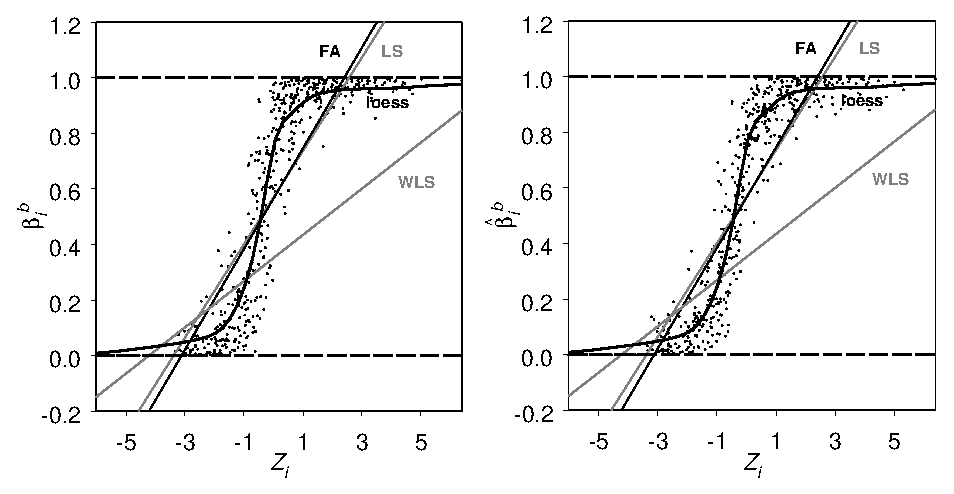
\epsfig{file=nonlinear.eps}
    \caption{Data with a Nonlinear Relationship.  Plot of $Z_i$ 
      horizontally by the estimated $\hat\beta_i^b$ vertically (in the
      right graph) and the true $\beta_i^b$ (in the left graph) with
      fits for least squares (LS) and our fully adjusted method (FA)
      almost on top of one another, weighted least squares (WLS), and
      the better fitting logistic transformation (LT).  Note how all
      the linear methods give out of bounds predictions.  Data were
      generated from the extended EI model, with
      $\breve\psi=(1.2,1,1.2,1,0.3,0.3,0)$, $X \sim \textrm{Uniform}(0,1)$, and
      $Z \sim \textrm{Normal}(0,2)$.}
    \label{f:nonlinear}
  \end{center}
\end{figure}

\section{Adjustments in Practice: A Replication of Burden and Kimball (1998)}

At least in some applications, differences among the various methods
of second stage analysis make little difference.  We replicate Burden
and Kimball's (1998) study of split-ticket voting, the empirical study
using second stage regressions on which HS focus the most, and find
that none of the proposed corrections affect the substantive
conclusions of the original study.  Table \ref{t:bkrep} presents these
results (assuming arguendo that every other feature of their model is
correctly specified).
\begin{table}[th]
\label{t:bkrep}
\begin{center}
\begin{tabular}{lcccccc}
& \multicolumn{3}{c}{\underbar{President/House}} & \multicolumn{3}{c}{\underbar{President/Senate}}\\
Variable        &       LS      &       FA      &       WLS     &       LS      &       FA      &       WLS     \\
\hline
Constant        &       0.066   &       -0.092  &       0.034   &       0.139   &       -0.016  &       0.167   \\
        &       (0.008) &               &       (0.014) &       (0.083) &               &       (0.100) \\
Ideological distance    &       -       &       -       &       -       &       -0.023  &       -0.031  &       -0.046  \\
        &               &               &               &       (0.039) &               &       (0.050) \\
Democratic incumbent    &       0.108   &       0.149   &       0.048   &       0.057   &       0.077   &       0.040   \\
        &       (0.015) &               &       (0.033) &       (0.051) &               &       (0.064) \\
Spending ratio  &       0.349   &       0.483   &       0.598   &       0.325   &       0.440   &       0.394   \\
        &       (0.021) &               &       (0.042) &       (0.092) &               &       (0.111) \\
Ballot format   &       -0.032  &       -0.045  &       -0.137  &       -0.049  &       -0.066  &       -0.060  \\
        &       (0.008) &               &       (0.014) &       (0.036) &               &       (0.046) \\
South   &       0.044   &       0.061   &       0.175   &       0.063   &       0.085   &       0.033   \\
        &       (0.009) &               &       (0.013) &       (0.051) &               &       (0.065) \\
$N$     &       361     &       361     &       361     &       32      &       32      &       32      \\
\hline
\end{tabular}
\end{center}
\caption{\em Replication of Burden and Kimball's study of ticket
  splitting.  The dependent variable is the estimated proportion of 
voters who split their tickets between the Republican presidential 
candidate and a Democratic Congressional candidate in the 1988 general 
election, obtained from EI.  LS denotes least squares estimates, FA 
full adjustment, and WLS weighted least squares.  Standard errors in 
parentheses.  This table replicates Burden and Kimball (1998) Table 
6, p. 539.}
\end{table}

Burden and Kimball investigated ticket-splitting behavior in the 1988
U.S. general election.  They used EI to estimate the proportion of
Bush voters who also voted for a Democratic Congressional candidate
(considering House and Senate separately), then employed these
estimates as dependent variables in second-stage regressions.  Their
goal was to show whether ticket splitting was the result of
intentional efforts by moderate voters to balance ideologically
disparate candidates (Alesina and Rosenthal, 1995) or an artifact of
differing campaign resources (Jacobson, 1997) and ballot formats
(Beck, 1997).  They found that ticket splitting falls with the
ideological distance between presidential and Senate candidates,
undermining the balancing thesis, but also that differences in
campaign resources appear to predict ticket splitting quite well.

Burden and Kimball's work is consistent with our recommendations.  The
relationship they examine is approximately linear, and few of the
bounds are particularly wide or narrow.  Appropriately, they report
both least squares and weighted least squares estimates, which we were
able to replicate reasonably well (see columns LS and WLS in Table
\ref{t:bkrep}).  We also computed our fully adjusted method (column
FA).\footnote{Since Burden and Kimball estimate their dependent
  variable using a two-stage EI procedure, we used only the second
  stage to compute the fully adjusted method.} In most cases, the FA
results are comparable to, or bracketed by, the LS and WLS estimates
(which Burden and Kimball considered sufficiently similar to use
interchangeably).  In particular, we obtain generally similar results
for the two most important variables in Burden and Kimball's model,
spending ratio and ideological distance.  All three methods thus
support Burden and Kimball's argument that ticket-splitting results
not from intentional balancing, but as an unintentional result of
campaign specific factors.

Note that Table \ref{t:bkrep} reports no standard errors for the fully
adjusted method, as HS offer no procedure for computing standard
errors for their adjusted coefficients.  It would be possible to
calculate standard errors for these estimates (by extending beyond
linear econometrics), although slightly complicated because the
adjusted estimators are ratios and also because the dependence of the
numerator and denomonator needs to be worked out.

\section{Concluding Suggestions}

As indicated in King (1997) and quoted above, ``The best first
approach is usually to display a scatterplot of the explanatory
variable (or variables) horizontally and (say) an estimate of
$\beta_i^b$ or $\beta_i^w$ vertically.  In many cases, this plot will
be sufficient evidence to complete the second stage analysis.''  This
key claim remains accurate.  Indeed \emph{show us the data} is a good
general motto for any statistical analysis, especially those with
complex nonlinear and bounded variables such as those resulting from
making ecological inferences.  To this scatterplot, we would suggest
adding information on the bounds.  This can be done by adding a thin
vertical line representing the bounds on $\beta_i^b$ for each
$(\hat\beta_i^b,Z_i)$ point plotted (e.g., King, 1997: Figure 13.2).
From this figure, we can then see all the data, precisely how
informative the bounds are, whether the bounds are of constant or
variable width.

For researchers who wish a simple approximation to estimating a second
stage relationship, the information provided in this article should
provide a guide to helping choose intelligently among the unadjusted,
adjusted, weighted, or nonlinear methods.  Researchers can easily tell
in which of the four prototypical situations listed and illustrated in
Section \ref{s:alt} their data fall, and they can take the action
indicated.

If a more formal statistical approach seems desirable, then a good
method must go beyond classical linear econometric theory.  It must
take into account (a) the nonlinear nature of the problem, (b) the
bounded nature of the second stage dependent variable with the width
of the bounds varying over observations, (c) the heteroskedasticity,
and (d) the effect of any possible logical inconsistency of the first
and second stages of the analysis (since two-step statistical methods
need not be logically consistent to work well; see, e.g., Meng, 1994).
At present, the only model that has been proposed with all these
properties is the extended EI model that allows covariates to be
included as part of the EI estimation procedure (King, 1997: Ch.9).
HS are correct that this extended model is sometimes only weakly
identified, but that is only when $X$ is included among the covariates
or highly related to $Z$.  In other cases, especially when $Z$ is
unrelated to $X$, the extended model will often be strongly identified
and so can be used without problem.  Imai and King (2002) demonstrate
how to compute first differences and other quantities of interest from
the extended EI model, and they report on extensions of the EI
software to make this possible.

Econometric theory and the classical linear regression framework works
well for what it was designed for.  However, in models with nonlinear
relationships or sample spaces or parameter spaces that are highly and
differentially bounded, such as in ecological inference problems,
political methodologists need to look elsewhere or develop their own
methods.  

HS have made an important contribution by highlighting the shrinkage
property of Bayesian point estimates like those provided by EI.  We
are in their debt for pointing this out and stimulating the ideas and
methods offered here.

\section*{References}
\mbox{} \baselineskip=6pt 
\parskip=1.5\baselineskip plus 4pt minus 4pt
\vspace{-\parskip}

\bibitem Alesina, Alberto and Howard Rosenthal.\ 1995.  \emph{Partisan
  Politics, Divided Government, and the Economy.}  New York: Cambridge
University Press.

\bibitem Beck, Paul Allen.\ 1997. \emph{Party Politics in America.}, 8th. ed.
Washington, DC: CQ Press.

\bibitem Burden, Barry C., and David C. Kimball.\ 1998.  ``A New Approach to
the Study of Ticket Splitting,'' \emph{American Political Science
  Review} 92, 3: 533--544.

\bibitem Jacobson, Gary C.\ 1990.  \emph{The Politics of Congressional
  Elections.} 4th ed.  New York: Longman.

\bibitem Meng, X.L.\ 1994. ``Multiple-imputation Inferences with Uncongenial
Sources of Input,'' \emph{Statistical Science}, 9, 4: 538--573.
\end{document}

